%**********************************************************************%
%  _               _____                    _       _
% | |   _   _  __ |_   _|__ _ __ ___  _ __ | | __ _| |_ ___
% | |  | | | |/ _` || |/ _ \ '_ ` _ \| '_ \| |/ _` | __/ _ \
% | |__| |_| | (_| || |  __/ | | | | | |_) | | (_| | ||  __/
% |_____\__,_|\__,_||_|\___|_| |_| |_| .__/|_|\__,_|\__\___|
%**********************************************************************%
% Version 1.0 of LuaTemplate, August 2024
%**********************************************************************%
% USAGE
% It also requires running UpBibTeX and UpMendex
% The commands are as follows:
%  1)  lualatex luatemplate.tex
%  2)  runluatemplate.bat または runluatemplate.command
%                   (Windows)                   (MaC)
%  3)  rmluatemplate.bat
% folder structure
%  luatemplate
%   │  apsrev4-2ja.bst
%   │  luatemplate.pdf
%   │  luatemplate.tex
%   │  mybib.bib
%   │  myist.ist
%   │  mysty.sty
%   │  rmluatemplate.bat
%   │  rmluatemplate.command
%   │  runluatemplate.bat
%   │  runluatemplate.command
%   │
%   ├─bib
%   │  │  doi2bib.py
%   │  │  mydoi.csv
%   │  │
%   │  └─doi2bib
%   │      │  crossref.py
%   │      │  __init__.py
%   │      │
%   │      └─bin
%   │            doi2bib
%   ├─code
%   │      bayes.sce.txt
%   │      template.py
%   │      template.vba
%   │
%   └─img
%          template.png
%**********************************************************************%
%                      _
%  _ __ ___  _   _ ___| |_ _   _
% | '_ ` _ \| | | / __| __| | | |
% | | | | | | |_| \__ \ |_| |_| |
% |_| |_| |_|\__, |___/\__|\__, |
%            |___/         |___/
%**********************************************************************%
% Version 1.0 of LuaTemplate, August 2024
\RequirePackage{plautopatch} %日本語パッケージを使う.
%**********************************************************************%
% ドキュメントクラス
%----------------------------------------------------------------------%
\documentclass[11pt,a4paper, titlepage]{ltjsarticle}
% USAGE
% - ltjsarticle, ltjsreport, ltjsbook
% - twocolumn: 2段組にする.
% - titlepage: \maketitle, apstractを単独ページにする.
% - draft: 校正用のオプション.
% ### book → articleへの変更は次のように置換する.
% ```
% \subsubsection → \subsubsubsection
% \subsection → \subsubsection
% \section → \subsection
% \chapter → \section
% ```
% 小さい順に格下げ
% ### book → articleへの変更は次のように置換する.
% ```
% \section → \chapter
% \subsection → \section
% \subsubsection → \subsection
% \subsubsubsection → \subsubsection
% ```
% 大きい順に格上げ.
% 
%**********************************************************************%
% ページ番号をフッターに表示
%----------------------------------------------------------------------%
\usepackage{fancyhdr}
\usepackage{lastpage} % フッタ中央に"今のページ数/総ページ数"を設定
\pagestyle{fancy}
\fancyhf{}
\fancyfoot{}

\makeatletter
\@ifclassloaded{ltjsarticle}{
  % ltjsarticleの場合の設定
  %\cfoot{\thepage~/~\pageref{LastPage}} %中央揃え"今のページ数/総ページ数"
  \cfoot{\thepage} %中央揃え"今のページ数"
  \renewcommand{\sectionmark}[1]{\markboth{第\ \thesection 章 \ #1}{}}
  \renewcommand{\subsectionmark}[1]{\markright{\thesubsection \ #1}}
  \fancyhead[L]{\leftmark}
  \fancyhead[R]{\rightmark}
  \let\origchapter\chapter
  \let\origsection\section
  \let\origsubsection\subsection
  \newcommand{\chapter}{\origsection}
  \renewcommand{\section}{\origsubsection}
  \renewcommand{\subsection}{\subsubsection}

}{
  \@ifclassloaded{ltjsbook}{
    % ltjsbookの場合の設定
    \fancyfoot[LE,RO]{\thepage}
    % ヘッダーに章と節を表示
    \renewcommand{\sectionmark}[1]{\markboth{第\ \thechapter 章 \ #1}{}}
    \renewcommand{\subsectionmark}[1]{\markright{\thesection \ #1}}
    \fancyhead[LE]{\leftmark} % 偶数ページのヘッダーに章を表示
    \fancyhead[RO]{\rightmark} % 奇数ページのヘッダーに節を表示
    \fancypagestyle{plainhead}{}
    \fancypagestyle{plainfoot}{}
    % TeXは米国規格のレターボックスサイズ(A4サイズより小さい)向けに
    % チューニングされており、1行の長さが全角40文字を超えないようにしている
    % 1行40文字の制限をなくすと左右に極端に寄ることがなくなる.
    \setlength{\fullwidth}{\oddsidemargin}
    \setlength{\oddsidemargin}{\evensidemargin}
    \setlength{\evensidemargin}{\fullwidth} %偶数ページの左余白を10mm(+1インチ)
    \setlength{\fullwidth}{\textwidth} %奇数ページの左余白を10mm(+1インチ
  }{
    \ClassError{preamble}{Unsupported document class}{Please use ltjsarticle or ltjsbook}
  }
}
\makeatother

%**********************************************************************%
% フォント
%----------------------------------------------------------------------%
\usepackage{luatexja} %日本語文書の組版を行う
\usepackage[T1]{fontenc} %アクセント記号をUTF-8で使用する. és viszlát! 
\usepackage{inconsolata-nerd-font} %等幅フォント consolas
%**********************************************************************%
% 数
%----------------------------------------------------------------------%
\usepackage{amsmath, amssymb} % 数式パッケージ
\usepackage{mathrsfs} %筆記体 $\mathscr{H}$ $\mathscr{L}$
\usepackage{bm} % for vector
%**********************************************************************%
% 図表
%----------------------------------------------------------------------%
\usepackage{here} %[H]オプション : 図表を文中のその場所に配置
\usepackage{ulem} % for \sout{} 取り消し線
\usepackage{booktabs} % \toprule \midrule \bottomrule
\usepackage{xcolor} %色
\usepackage{comment} %\begin{comment} \end{comment}でコメントアウト
\usepackage{boites} %ボックス内で改ページ可 
%**********************************************************************%
% 参照
%----------------------------------------------------------------------%
\usepackage{url} %URL をタイプライタ体で出力する\url{http://}
\usepackage[unicode=true,hidelinks,bookmarksnumbered=true,
bookmarksdepth=subsubsection]{hyperref}
% しおりをつけるには\label{sec:}を1回以上使わなければならない.
\hypersetup{colorlinks=true,citecolor=blue,linkcolor=blue,urlcolor=blue}
\usepackage[sort&compress,numbers]{natbib}
\usepackage{doi} %apsrev4-2jaを使うのに必要
%**********************************************************************%
% 装飾
%----------------------------------------------------------------------%
\usepackage{ascmac} %キートップ
\let\OldReturn\Return % ascmacのReturnコマンドを別の名前に保存
\usepackage{pxrubrica} %ルビを使う. 例) 尤度\ruby{ゆう|ど}
\usepackage{tcolorbox} %枠囲み
%**********************************************************************%
% レイアウト
%----------------------------------------------------------------------%
\usepackage{fancyhdr} %レイアウトで使う
\usepackage[absolute,overlay]{textpos} % 絶対位置指定 レイアウトで使う
\usepackage{array}  % 表幅固定
\usepackage{multirow}   % 表で行結合

%**********************************************************************%
% 索引 theindex 環境
%----------------------------------------------------------------------%
\usepackage{makeidx}
\makeindex
%**********************************************************************%
% デバグ
%----------------------------------------------------------------------%
\usepackage{layout} %\layout 現在のレイアウトの確認
\usepackage{lipsum} %ダミーテキスト
%**********************************************************************%
\makeatletter                   % プリアンブルで定義開始
% 表示文字列を"図"から"Figure"へ
\renewcommand{\figurename}{図 }
\renewcommand{\tablename}{表 }
% 図番号を"<節番号>.<図番号>" へ
\renewcommand{\thefigure}{\thesection.\arabic{figure}}
\renewcommand{\thetable}{\thesection.\arabic{table}}
\renewcommand{\theequation}{\thesection.\arabic{equation}}
% 節が進むごとに図番号をリセットする
\@addtoreset{figure}{section}
\@addtoreset{table}{section}
\@addtoreset{equation}{section}
\newcommand{\記}{\begin{center} 記 \end{center}}
\newcommand{\挨拶}{\noindent 拝啓 \ifcase\month\or 厳寒\or 春寒\or 早春
    \or 陽寒\or 新緑\or 向暑\or 猛暑\or 残暑\or 初秋\or 仲秋\or 晩秋\or 初冬
    \fi の候, ますますご清栄のこととお喜び申し上げます.}
\newcommand{\refSec}[1]   {\ref{#1}章}
\newcommand{\refApd}[1]   {\ref{#1}}
\newcommand{\refSsec}[1]  {\ref{#1}節}
\newcommand{\refSssec}[1] {\ref{#1}項}
\newcommand{\refFig}[1]   {\figurename\ref{#1}}
\newcommand{\refTable}[1] {\tablename\ref{#1}}
\newcommand{\refEq}[1]    {Eq \ref{#1}}
\newcommand{\refCode}[1]    {Lisging \ref{#1}}
\newcommand{\refAlgorithm}[1]    {Algorithm \ref{#1}}
\newcommand*\rfrac[2]{{}^{#1}\!/_{#2}}
\newcommand{\mybib}[7]{\bibitem{#1}{\href{#2}{#3, #4, {\bf #5}(#6)#7}}}
%図の挿入\myfig{ワイド[cm]}{ファイル名}{キャプション}
\newcommand{\myfig}[3]{\begin{figure}[H]\centering\includegraphics
    [clip, width=#1cm]{./img/#2}\caption{#3\label{fig:#2}}\end{figure}}
%表の挿入\mytable{lcc}{ヘッダー}{内容}{キャプション}{ラベル}
\newcommand{\mytable}[5]{\begin{table}[H] \centering 
    \renewcommand{\arraystretch}{0.8} \begin{tabular}{#1} 
        \toprule #2 \midrule #3 \bottomrule \end{tabular} 
        \caption{#4 \label{#5}} \renewcommand{\arraystretch}{1} \end{table}}
%式の挿入\myeq{}
\newcommand{\myeq}[2]{\begin{eqnarray}#1\label{eq:#2}\end{eqnarray}}
\newcommand{\myce}[1]{$\rm{#1}$}
% newenvironment
\newenvironment{記2}
{\begin{center} 記 \end{center}\begin{description}}
        {\end{description}}
\makeatother % プリアンブルで定義終了
%**********************************************************************%
% ソースコード
%----------------------------------------------------------------------%
\usepackage{xcolor}
\definecolor{deepgreen}{rgb}{0, 0.502, 0}
\definecolor{deepyellow}{rgb}{0.502, 0.502, 0}
\definecolor{deepcyan}{rgb}{0, 0.502, 0.502}
\definecolor{deepmagenta}{rgb}{0.502, 0, 0.502}
\definecolor{orange}{rgb}{1, 0.502, 0}
\usepackage{listings}

\lstdefinestyle{Python}{
    language        = Python,
    morekeywords=[1]{   % 予約語 標準ライブラリを含む
            False,None,True,and,as,assert,
            async,await,break,class,continue,def,
            del,elif,else,except,finally,for,
            from,global,if,import,in,is,
            lambda,nonlocal,not,or,pass,raise,
            return,try,while,with,yield,
        },
    basicstyle      = \ttfamily\gtfamily,
    % identifierstyle = \color{deepcyan}, %定数
    keywordstyle    = [1]\color{blue},
    stringstyle     = \color{red},
    commentstyle    = \color{deepgreen},
    columns=fixed,
    basewidth=0.7em,
    showstringspaces=false,
    frame       = single,
    numbers     = left,
    showspaces  = false,
    showstringspaces    = false,
    captionpos  = t,
    caption     = \lstname,
}


\lstdefinestyle{VBA}{
    language={[Visual]Basic},
    morekeywords=[1]{   % 予約語 標準ライブラリを含む
            Abs,AddressOf,And,Any,Array,
            As,Attribute,Boolean,ByRef,Byte,
            ByVal,Call,Case,Cbool,Cbyte,
            Ccur,Cdate,CDbl,Cdec,Cdecl,
            Cint,Circle,CLng,CLngLng,CLngPtr,
            Close,Const,CSng,CStr,Currency,
            CVar,CVErr,Date,Debug,Decimal,
            Declare,DefBool,DefByte,DefCur,DefDate,
            DefDbl,DefDec,DefInt,DefLng,DefLngLng,
            DefLngPtr,DefObj,DefSng,DefStr,DefVar,
            Dim,Do,DoEvents,Double,Each,
            Else,ElseIf,empty,End,EndIf,
            Enum,Eqv,Erase,Event,Exit,
            False,Fix,For,Friend,Function,
            Get,Global,GoSub,GoTo,If,
            Imp,Implements,In,Input,InputB,
            Int,Integer,Is,Lbound,Len,
            LenB,Let,Like,LINEINPUT,Lock,
            Long,LongLong,LongPtr,Loop,Lset,
            Me,Mod,New,Next,Not,
            nothing,null,On,Open,Option,
            Optional,Or,ParamArray,Preserve,Print,
            Private,PSet,Public,Put,RaiseEvent,
            ReDim,Rem,Resume,Return,Rset,
            Scale,Seek,Select,Set,Sgn,
            Shared,Single,Spc,Static,Stop,
            String,Sub,Tab,Then,To,
            True,Type,TypeOf,Ubound,Unlock,
            Until,Variant,VB_Base,VB_Control,VB_Creatable,
            VB_Customizable,VB_Description,VB_Exposed,VB_Ext_KEY,VB_GlobalNameSpace,
            VB_HelpID,VB_Invoke_Func,VB_Invoke_Property,VB_Invoke_PropertyPut,VB_Invoke_PropertyPutRefVB_MemberFlags,
            VB_Name,VB_PredeclaredId,VB_ProcData,VB_TemplateDerived,VB_UserMemId,
            VB_VarDescription,VB_VarHelpID,VB_VarMemberFlags,VB_VarProcData,VB_VarUserMemId,
            Wend,While,With,WithEvents,Write,
        },
    basicstyle      = \ttfamily\gtfamily,
    keywordstyle    = [1]\color{blue},
    stringstyle     = \color{red},
    commentstyle    = \color{deepgreen},
    columns=fixed,
    basewidth=0.7em,
    showstringspaces=false,
    frame       = single,
    numbers     = left,
    showspaces  = false,
    showstringspaces    = false,
    captionpos  = t,
    caption     = \lstname,
}

%**********************************************************************%
% アルゴリズム
%----------------------------------------------------------------------%
\usepackage[linesnumbered,ruled,vlined]{algorithm2e}
\let\algorithmReturn\Return % algorithm2eのReturnコマンドを新しい名前に定義
\DontPrintSemicolon
% Define pseudocode formatting
\renewcommand{\KwSty}[1]{\textnormal{\textcolor{blue!90!black}{\ttfamily\bfseries #1}}\unskip}
\renewcommand{\ArgSty}[1]{\textnormal{\ttfamily #1}\unskip}
\SetKwComment{Comment}{\color{green!50!black}// }{}
\renewcommand{\CommentSty}[1]{\textnormal{\ttfamily\color{green!50!black}#1}\unskip}
\newcommand{\assign}{\leftarrow}
\newcommand{\var}{\texttt}
\newcommand{\FuncCall}[2]{\texttt{\bfseries #1(#2)}}
\SetKwProg{Function}{function}{}{}
\renewcommand{\ProgSty}[1]{\texttt{\bfseries #1}}
\usepackage{graphicx}
\renewcommand{\thefootnote}{\arabic{footnote}}

%**********************************************************************%
%      _                                       _
%   __| | ___   ___ _   _ _ __ ___   ___ _ __ | |_
%  / _` |/ _ \ / __| | | | '_ ` _ \ / _ \ '_ \| __|
% | (_| | (_) | (__| |_| | | | | | |  __/ | | | |_
%  \__,_|\___/ \___|\__,_|_| |_| |_|\___|_| |_|\__|
%**********************************************************************%
\begin{document}
%**********************************************************************%
% タイトル
%----------------------------------------------------------------------%
% \title{Lua\LaTeX\index{lualatex} テンプレート\footnote{本書の記載内容は情報使用の目的で提供される. 記載内容は予告なく変更することがあり, その内容については筆者のせきにんとはみなされない. 本書にきさいされている情報の正確性および信頼性には万全を期しているが, 本書における誤りや不正確な情報により生じる損害に関して, また,
%         コードを利用して得られた文書への責任ン位関して著者は一切の責任を持たない.
%         \\本書の内容はWindows11, Mac Sonomaで動作確認をしている.
%         \\本書の内容は著作権法上の保護を上kる. 著者の文書による承認を得ずに,
%         本書の内容の一部, あるいは全部を無断で複写(コピー)・複製・転載することを禁ずる.}
%     \\第1版}
% 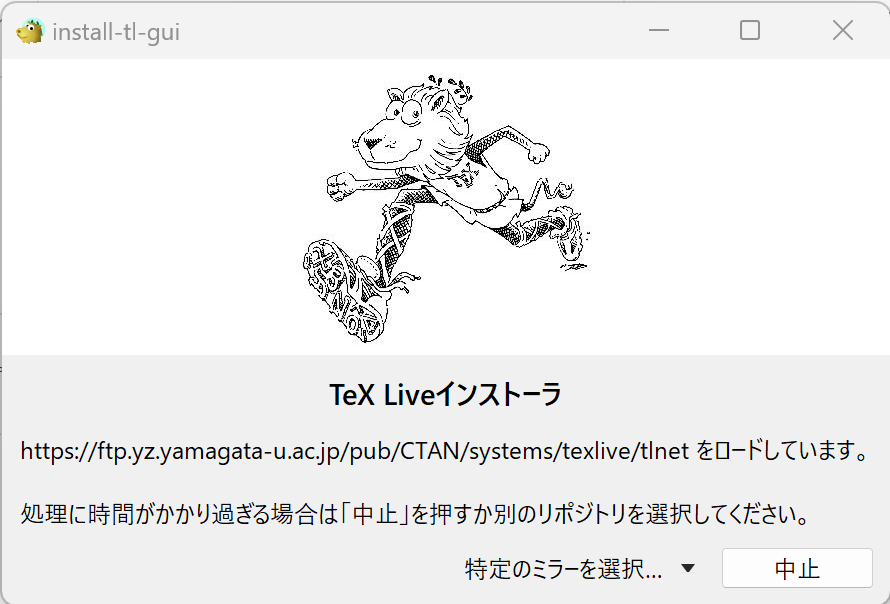
\includegraphics[width=0.1\textwidth]{img/template.png}
% \author{名前太郎\thanks{名前太郎の所属} \and 名前次郎\thanks{名前次郎の所属}}
% \date{\today}
% \maketitle
\begin{titlepage}
    \centering
    \vspace*{\fill}
    \Huge{\textbf{{Lua\LaTeX\index{lualatex} テンプレート\footnote{本書の記載内容は情報使用の目的で提供される. 記載内容は予告なく変更することがあり, その内容については筆者のせきにんとはみなされない. 本書にきさいされている情報の正確性および信頼性には万全を期しているが, 本書における誤りや不正確な情報により生じる損害に関して, また、コードを利用して得られた文書への責任ン位関して著者は一切の責任を持たない. \\本書の内容はWindows11, Mac Sonomaで動作確認をしている. \\本書の内容は著作権法上の保護を上kる. 著者の文書による承認を得ずに, 本書の内容の一部, あるいは全部を無断で複写(コピー)・複製・転載することを禁ずる.} \\第1版}}} \\
    \large{名前太郎\footnote{名前太郎の所属}, 名前次郎\footnote{名前次郎の所属}} \\
    \large{\today} \\
    \vspace*{\fill}
    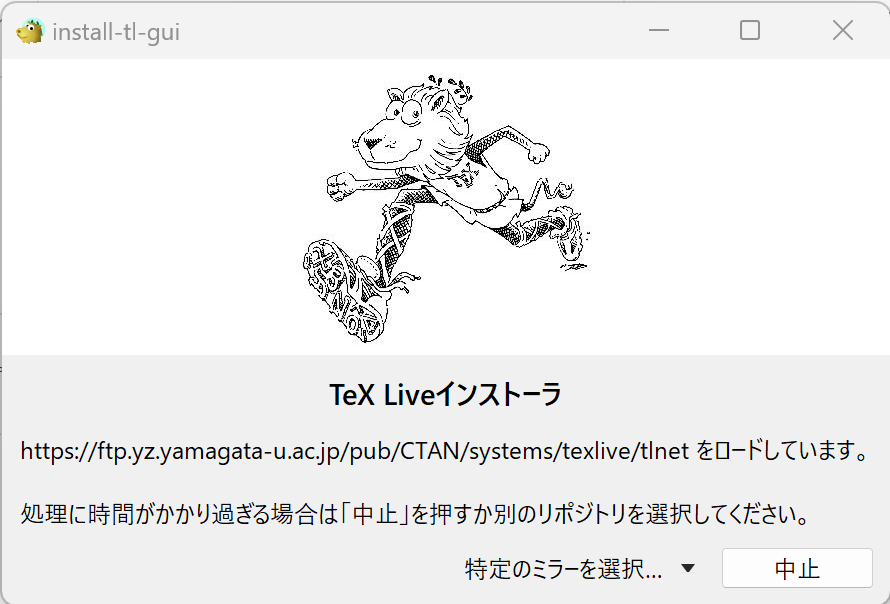
\includegraphics[width=0.4\textwidth]{img/template.png}
\end{titlepage}

%**********************************************************************%
% 本文より前のページ数はローマ数字とする.
%----------------------------------------------------------------------%
\pagenumbering{roman}
%**********************************************************************%
% 概要
%----------------------------------------------------------------------%
\begin{abstract}
    <<<<<<< HEAD
    \lipsum[1-2]
    =======
    \lipsum[1-10]
    >>>>>>> 4609bac839c02d6d33443e5e9e76761674de622f
\end{abstract}

%**********************************************************************%
% 目次
%----------------------------------------------------------------------%
\tableofcontents
\newpage
\listoffigures
\newpage
\listoftables
\newpage
%**********************************************************************%
% 本文のページ数はアラビア数字とする.
%----------------------------------------------------------------------%
\pagenumbering{arabic}
\makeatletter
\@ifclassloaded{ltjsarticle}{
    \cfoot{\thepage~/~\pageref{LastPage}}
}
\makeatother
%**********************************************************************%
% ダミー本文
%----------------------------------------------------------------------%
%\part{部の名前}
\chapter{ダミー章}
\lipsum[1-5]
\section{ダミー節 \label{sec:1}}
\lipsum[6-20]
\lipsum[21-25]
\paragraph{ダミーパラグラフ}
\lipsum[20]
\subsection{ほげ}

\chapter{フォント・装飾}
%**********************************************************************%
% フォント
%----------------------------------------------------------------------%
\section{フォント}
\textbf{ボールド} \par
\textit{Italic} \par
\small{フォント小さい} \par
\large{フォント大きい} \par
\fbox{文字を囲む.} \par
\texttt{Typewriter} \par
\textgt{ゴシック} \par
\keytop{キートップ} \par
%**********************************************************************%


%**********************************************************************%
% 数式
%----------------------------------------------------------------------%
\section{数式}
$T_{\rm N1}\,{=}\,0.97~{\rm K}$
$H\,{-}\,T$
$J_1^{\prime}$
$H_{\rm s}$
\myeq{x=y}{1}
%**********************************************************************%
% 枠
%----------------------------------------------------------------------%
\section{枠}
\begin{tcolorbox}[colframe=black, colback=white,
        colbacktitle=blue, coltitle=white,
        fonttitle=\bfseries\sffamily,title=
        純粋な枠]
    わくわく
\end{tcolorbox}

\begin{breakbox}
    \begin{itemize}
        \item folder\\folder2
        \item folder\\folder3
        \item folder\\folder4
    \end{itemize}
\end{breakbox}

本書で用いるプログラムはかなり多く, 目まぐるしく変わる.
そこで円滑な進行を図るとともにその内容に遺漏がないように
Windows上での操作手順を逐一記述しておく.
料理のレシピに相当する.
以後, 本文書では次の表記
\begin{screen}
    \begin{table}[H]
        \centering
        \renewcommand{\arraystretch}{0.8}
        \begin{tabular}{ll}
            「・・・」              & : プルダウンメニュー(>は階層同士の区切り)              \\
            "・・・"              & : ダイアログやメニュー中の設定・チェック項目, 質問, 一般の文字列. \\
            \lbrack ・・・\rbrack & : ボタン.                               \\
            \textbf{ボールド書体}    & : マクロ, ファイル名.                        \\
            \keytop{・・・}       & : キートップ.                             \\
        \end{tabular}
        \renewcommand{\arraystretch}{1}
    \end{table}
\end{screen}
を採用するものと約束する. 特筆大書したい文を\textcolor{red}{赤文字}で表示した.
慣習に従い, "hoge" はファイル名から拡張子を除いた文字列(メタ構文変数)
を表すものと約束する.
%**********************************************************************%
% 箇条書き
%----------------------------------------------------------------------%
\section{箇条書き}
\begin{itemize}
    \item 箇条書き
\end{itemize}

\begin{enumerate}
    \item 箇条書き
\end{enumerate}

%**********************************************************************%
% 参照
%----------------------------------------------------------------------%
\section{参照}
\refFig{fig:template.png}\par
\refTable{table:1}\par
\refSec{sec:1}\par
\refEq{eq:1}\par
\refApd{apd:1}\par
\refCode{code:1}\par
\refAlgorithm{algorithm:1} \par
\hypertarget{square}{正方格子}\par
\hyperlink{square}{正方格子}\par
\href{http://hoge}{url}\par
\url{http://hoge}\par
\cite{Plumer_1988} \par
\cite{Plumer_1989} \par
脚注を付けたい箇所\footnote{これが脚注です.}.
%**********************************************************************%
\chapter{図・表}
%**********************************************************************%
% 図
%----------------------------------------------------------------------%
\myfig{12}{template.png}{キャプションです.}
%**********************************************************************%
% 表
%----------------------------------------------------------------------%
\mytable{lcc}
{\textbf{1} & \textbf{1} & \textbf{1} \\ }
{\textbf{1} & 1  & 1  \\ }
{キャプション}
{table:1}


%**********************************************************************%
% ソースコード
%----------------------------------------------------------------------%
\chapter{ソースコード} %プログラムファイルをインポートする.
\lstinputlisting[style=Python, caption = PythonによるFizzBuzzのコード.,label = code:1]{code/template.py}
\lstinputlisting[style=VBA, caption = VBAによるFizzBuzzのコード.,label = code:1]{code/template.vba}



%**********************************************************************%
% アルゴリズム
%----------------------------------------------------------------------%
\begin{algorithm}
    \label{algorithm:1}
    \caption{Dynamic PCA}
    \Comment{$\theta_{\mathrm{exp}}$ is globally given,
        and initially set to $\infty$.}
    \Function{ExpandBasisIfInteresting($B$, $\Sigma$, $\vec{x}$)}{
        \If{$\var{loss} > \theta_{\mathrm{exp}}$}{
            $\var{loss} \assign
                \sqrt{\lVert \vec{x} \rVert^2 - \lVert \vec{x}^T B \rVert^2}$
            \Comment{By Pythagoras}
            $B, \Sigma \assign
                \FuncCall{Append}{$B$, $\Sigma$, $\vec{x}$}$\;
            $B \assign \FuncCall{GramSchmidt}{$B$}$\;
        }
        $\theta_{\mathrm{exp}} \assign
            \FuncCall{UpdateLoss}{$\theta_{\mathrm{exp}}$, \var{loss}}$\;
        \algorithmReturn{$B$, $\Sigma$}\;
    }
    \Function{PeriodicDecompose($B$, $\Sigma$)}{
        \If{\FuncCall{IsOneMinutePassed}{}}{
            $B, \Sigma \assign \FuncCall{PCA}{$B$, $\Sigma$}$\;
        }
        \algorithmReturn{$B$, $\Sigma$}\;
    }
    \Comment{The main function}
    \Function{DynPCA($B$, $\Sigma$, $\vec{x}$, $s$)}{
        $B, \Sigma \assign
            \FuncCall{ExpandBasisIfInteresting}{$B$, $\Sigma$, $\vec{x}$}$\;
        $\Sigma \assign
            \FuncCall{UpdateCovMatrix}{$B$, $\Sigma$, $\vec{x}$, $s$}$\;
        $B', \Sigma' \assign
            \FuncCall{PeriodicDecompose}{$B$, $\Sigma$}$\;
        \algorithmReturn{$B'$, $\Sigma'$}
    }
\end{algorithm}


%**********************************************************************%
% 索引
%----------------------------------------------------------------------%
\chapter{索引}
If you want convert TeX file to PDF file,
using lualatex\index{lualatex} is the greatest choice.
免疫\index{めんえき@免疫}とは,例外をおそれずにいえば,体内に入ってきた細菌や
ウィルス(非自己\index{ひじこ@非自己}
\footnote{抗原\index{こうげん@抗原}と総称される。})
といった自己にとって危険な要素を徹底的に排除しようと試みる際に,
脳以上に主導権を握っている
生体防御機構\index{せいたいぼうぎょきこう@生体防御機構}である。index{.ist}
\index{しいたいぼうぎょきこう@し体防御機構}
%**********************************************************************%
% 参考文献
%----------------------------------------------------------------------%
\newpage
\chapter{出典・参考文献}
\bibliographystyle{apsrev4-2ja}
\bibliography{mybib}

%**********************************************************************%
% 付録
%----------------------------------------------------------------------%
\appendix
\chapter{付録タイトル \label{apd:1}}
\section{付録見出し}

%**********************************************************************%
% 索引
%----------------------------------------------------------------------%
\newpage
\printindex  % この行を追加


%**********************************************************************%
% 奥付
%----------------------------------------------------------------------%
\begin{screen}
    {\Large Lua\LaTeX テンプレート 第1版} 定価はカバーに表示\\
    {\today 第1版}
    \begin{table}[H]
        \centering
        \renewcommand{\arraystretch}{0.8}
        \begin{tabular}{ll}
            著者 & 名前太郎 \\
               & 名前次郎 \\
        \end{tabular}
        \renewcommand{\arraystretch}{1}
    \end{table}
    ©2024<無題複写・転載を禁ず>
\end{screen}
%**********************************************************************%
\end{document}